\section{Research method} \label{sec_research_method}

This research is a Design Science Method and relies on the Engineering Cycles as described
by \textcite{wieringa_design_2014}. The engineering cycle provides a structured approach
to develop the required artifacts to analyze the design problem.

\begin{figure}[H]
    \centering
    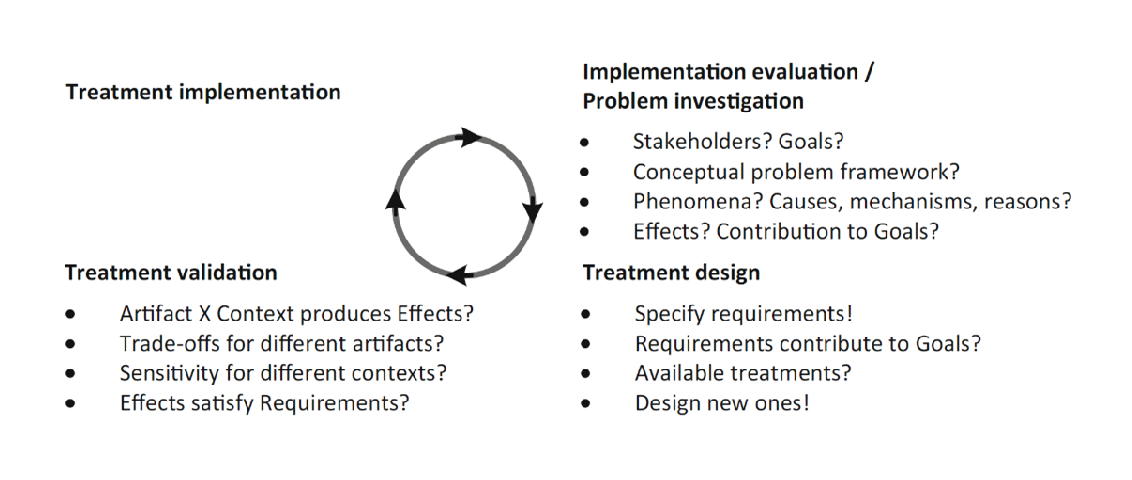
\includegraphics[width=1\textwidth]{Figures/engineering_cycle.pdf}
    \caption[Engineering cycle]{The Engineering Cycle of \textcite{wieringa_design_2014}}
    \label{fig_engineering_cycle}
\end{figure}

In the context of this research, the artifacts described in chapters
\ref{sec_generator_artifact} and \ref{sec_generated_artifact} are considered to be
information systems. \citeauthor{hevner_design_2004} proposed a framework for research
in information systems by introducing the interacting relevance and rigor cycles.

Figure \ref{fig_dsr} depicts a specialization of the Design Science Framework of
\textcite{hevner_design_2004}. The rigor cycle is composed of the theories and knowledge
from \gls{ns} and \gls{ca}. This is supplemented by the rigorous knowledge of modularity,
evolvability, and stability of software systems. The relevance cycle represents the
business needs of the stakeholders. The research requirements are described as research
objectives.

\begin{figure}[H]
    \centering
    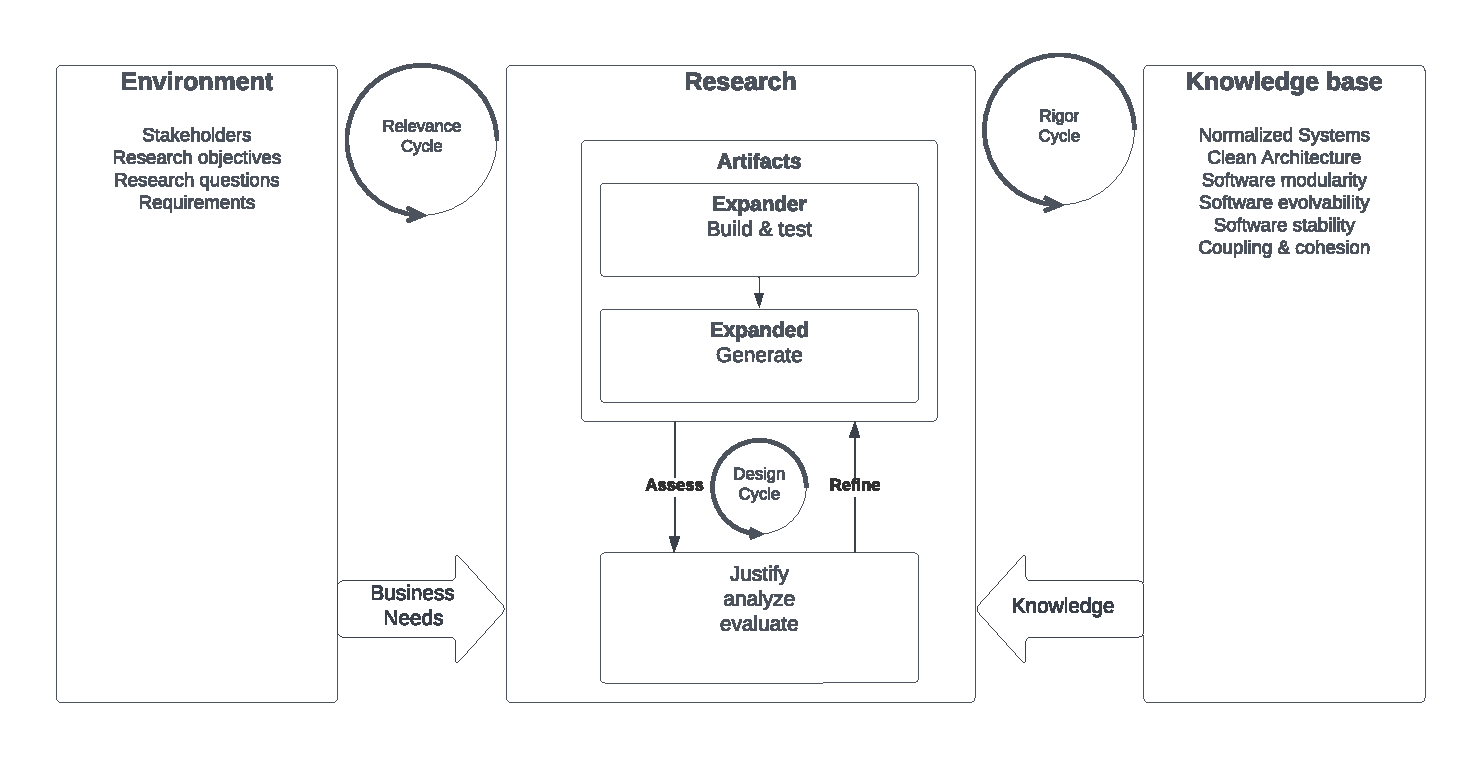
\includegraphics[width=1\textwidth]{Figures/rigor_relevance_cycle.pdf}
    \caption[Design Science Framework for IS Research]{The Design Science Framework for IS Research}
    \label{fig_dsr}
\end{figure}